\documentclass[12pt,letterpaper]{article}
\setcounter{page}{0}

\usepackage{bbm}
\usepackage{hhline}
\usepackage[multiple]{footmisc}
\usepackage{floatpag,amsmath,amsthm,amssymb}
\usepackage{changepage}

% Figure panel header font
\newcommand{\panel}{\fontfamily{phv}\selectfont\scriptsize\textbf}
\usepackage{amsmath} 
\DeclareMathOperator*{\argmin}{arg\,min}
\DeclareMathOperator*{\argmax}{arg\,max}


%%%%%%%%%%%%%%%%%%%%%%%%%%%%%%%
%% LOAD LOCAL COMPILATION PATHS
%%%%%%%%%%%%%%%%%%%%%%%%%%%%%%%
\newcommand{\HOME}{\string~}

% set input paths
\newcommand{\includepath}{.}
\newcommand{\shrugpath}{.}

% include standard package
\usepackage[latin1]{inputenc}
\usepackage{setspace}
\usepackage{amsmath}
\usepackage{amsthm}
\usepackage{amsfonts}
\usepackage{longtable}
\addtolength{\textwidth}{5cm}
\addtolength{\textheight}{5cm}
\usepackage{fullpage}
\usepackage{amssymb}
\usepackage[colorlinks=true]{hyperref}
\usepackage{url}
\usepackage{graphicx}
\usepackage{epstopdf}
\usepackage{multirow}
\usepackage{array}
\usepackage{harvard}
\usepackage{tabularx}
\citationmode{abbr}

\usepackage{float}
% \usepackage{perpage}
% \MakeSorted{figure}
% \MakeSorted{table}
\usepackage{lscape}
\usepackage{verbatim}
\usepackage{pdflscape}
\usepackage{chngcntr}
\usepackage{appendix}
\usepackage{booktabs,calc}
\usepackage{ulem}

% allow yellow highlighting in tables
\usepackage{color,colortbl}
\usepackage{soul}
\definecolor{Yellow}{rgb}{.88,1,.65}
\definecolor{Green}{rgb}{.65,1,.65}
\definecolor{Red}{rgb}{1,.65,.65}

\citationstyle{dcu}

\usepackage[labelfont=bf,center,large,labelsep=newline]{caption}
\usepackage{subfig}
% \counterwithout{subtable}{table}
\def\changemargin#1#2{\list{}{\rightmargin#2\leftmargin#1}\item[]}
\let\endchangemargin=\endlist

% define subscript / superscript commands
\newcommand{\superscript}[1]{\ensuremath{^{\textrm{#1}}}}
\newcommand{\subscript}[1]{\ensuremath{_{\textrm{#1}}}}

% create a shortcut for newlines in captions:
\newcommand{\cnewline}{\hspace{\linewidth}}

%format paper to save trees
\usepackage[right=1in,left=1in,top=1in,bottom=1in]{geometry}
\usepackage{savetrees}

%AER style headers
\def\thesection{\arabic{section}}
\def\thesubsection {\thesection.\arabic{subsection}}

% set home path
\newcommand{\HOME}{\string~}


% disable hyperlinks, which were breaking on appendix references
\usepackage[options]{nohyperref}

\title{Development Research at High Geographic Resolution: \\ An
  Analysis of Night Lights, Firms, and Poverty in India \\ using the
  SHRUG Open Data Platform}

\author{ \\ Sam Asher \\ Tobias Lunt \\ Ryu Matsuura \\ Paul Novosad \\ }

%%%%%%%%%%%%%%%%%%%%%% 
% TITLE PAGE
%%%%%%%%%%%%%%%%%%%%%% 
\begin{document}
\date{}
\maketitle \\ \\

\begin{center}
{\large Online Appendix: Additional Tables and Figures}
\end{center}

\begin{appendix}


%%%%%%%%%%%%%%%%%%%%%%%%%%%%%%%%%
%% APPENDIX TABLES AND FIGURES %%
%%%%%%%%%%%%%%%%%%%%%%%%%%%%%%%%%
\clearpage
\setcounter{pag}{1} \doublespacing

% reset table/figure numbers and prefix with A
\setcounter{table}{0}
\renewcommand{\thetable}{S\arabic{table}}
\setcounter{figure}{0}
\renewcommand{\thefigure}{S\arabic{figure}}


%%%%%%%%%%%%%%%%%%%%%%%%%%%%%%%%%%%%%%%%%%%%%%%%%%
%% table: population share matched to the SHRUG %%
%%%%%%%%%%%%%%%%%%%%%%%%%%%%%%%%%%%%%%%%%%%%%%%%%%
%\begin{landscape}
  \begin{table}[H]
    \caption{Population Share Matched to the SHRUG, by State} 
    \vspace{-5mm}

    \begin{center}
      \tiny{\setlength{\linewidth}{.1cm} \begin{center}
\newcommand{\contents}{\begin{tabular}{l|c|c|c}
\hline\hline
States & PC91 & PC01 & PC11 \\
\hline
India                    & 826117.89 / 833122.68 (99\%) & 1028120.50 / 1028349.73 (100\%) & 1209944.68 / 1210741.69 (100\%) \\
\hline
Andaman Nicobar Islands  & 280.66 / 280.66 (100\%) & 356.15 / 356.15 (100\%) & 380.55 / 380.58 (100\%) \\
Andhra Pradesh           & 65140.70 / 66455.27 (98\%) & 76210.01 / 76210.01 (100\%) & 84580.78 / 84580.78 (100\%) \\
Arunachal Pradesh        & 621.18 / 637.04 (98\%) & 1097.97 / 1097.97 (100\%) & 1383.17 / 1383.73 (100\%) \\
Assam                    & 22278.90 / 22311.78 (100\%) & 26640.04 / 26655.53 (100\%) & 30999.61 / 31205.58 (99\%) \\
Bihar                    & 86119.25 / 86374.47 (100\%) & 82825.55 / 82825.55 (100\%) & 104099.45 / 104099.46 (100\%) \\
\hline
Chandigarh               & 642.01 / 642.01 (100\%) & 900.63 / 900.63 (100\%) & 1055.45 / 1055.45 (100\%) \\
Chhattisgarh             & & 20827.74 / 20833.80 (100\%) & 25544.25 / 25545.20 (100\%) \\
Dadra Nagar Haveli       & 138.48 / 138.48 (100\%) & 220.49 / 220.49 (100\%) & 343.71 / 343.71 (100\%) \\
Daman \& Diu             & 101.59 / 101.59 (100\%) & 158.20 / 158.20 (100\%) & 243.25 / 243.25 (100\%) \\
Goa                      & 1155.51 / 1169.79 (99\%) & 1347.67 / 1347.67 (100\%) & 1458.55 / 1458.55 (100\%) \\
\hline
Gujarat                  & 41284.77 / 41309.58 (100\%) & 50671.02 / 50671.02 (100\%) & 60439.69 / 60439.69 (100\%) \\
Haryana                  & 16285.72 / 16459.98 (99\%) & 21139.38 / 21144.56 (100\%) & 25193.50 / 25351.46 (99\%) \\
Himachal Pradesh         & 5165.07 / 5170.53 (100\%) & 6077.90 / 6077.90 (100\%) & 6864.45 / 6864.60 (100\%) \\
Jammu Kashmir            & & 10142.76 / 10143.70 (100\%) & 12539.86 / 12541.30 (100\%) \\
Jharkhand                & & 26945.83 / 26945.83 (100\%) & 32983.76 / 32988.13 (100\%) \\
\hline
Karnataka                & 44663.16 / 44977.20 (99\%) & 52785.20 / 52850.56 (100\%) & 61032.42 / 61095.30 (100\%) \\
Kerala                   & 28631.18 / 29098.52 (98\%) & 31841.37 / 31841.37 (100\%) & 33406.06 / 33406.06 (100\%) \\
Lakshadweep              & 51.71 / 51.71 (100\%) & 60.65 / 60.65 (100\%) & 64.47 / 64.47 (100\%) \\
Madhya Pradesh           & 62281.73 / 63026.21 (99\%) & 60345.27 / 60348.03 (100\%) & 72626.81 / 72626.81 (100\%) \\
Maharashtra              & 78363.48 / 78936.42 (99\%) & 96878.63 / 96878.63 (100\%) & 112323.51 / 112374.34 (100\%) \\
\hline
Manipur                  & 1806.38 / 1837.15 (98\%) & 2166.79 / 2166.79 (100\%) & 2851.43 / 2855.79 (100\%) \\
Meghalaya                & 1764.66 / 1774.74 (99\%) & 2288.95 / 2318.82 (99\%) & 2961.91 / 2966.89 (100\%) \\
Mizoram                  & 689.54 / 689.76 (100\%) & 888.57 / 888.57 (100\%) & 1094.51 / 1097.21 (100\%) \\
Nagaland                 & 1207.14 / 1209.55 (100\%) & 1989.66 / 1990.04 (100\%) & 1978.50 / 1978.50 (100\%) \\
NCT of Delhi             & 9420.64 / 9420.64 (100\%) & 13850.51 / 13850.51 (100\%) & 16787.94 / 16787.94 (100\%) \\
\hline
Odisha                   & 31515.51 / 31587.64 (100\%) & 36799.75 / 36804.66 (100\%) & 41945.54 / 41969.76 (100\%) \\
Puducherry               & 771.56 / 807.78 (96\%) & 974.35 / 974.35 (100\%) & 1247.95 / 1247.95 (100\%) \\
Punjab                   & 19053.16 / 19053.16 (100\%) & 24334.90 / 24359.00 (100\%) & 27650.20 / 27743.34 (100\%) \\
Rajasthan                & 43354.10 / 43879.50 (99\%) & 56502.28 / 56507.19 (100\%) & 68548.43 / 68548.44 (100\%) \\
Sikkim                   & 405.02 / 405.02 (100\%) & 540.85 / 540.85 (100\%) & 610.57 / 610.58 (100\%) \\
\hline
Tamil Nadu               & 55111.89 / 55834.15 (99\%) & 62367.39 / 62405.68 (100\%) & 72117.59 / 72147.03 (100\%) \\
Tripura                  & 2430.67 / 2757.20 (88\%) & 3198.93 / 3199.20 (100\%) & 3666.08 / 3673.92 (100\%) \\
Uttarakhand              & & 166186.02 / 166197.92 (100\%) & 199763.41 / 199812.34 (100\%) \\
Uttar Pradesh            & 138452.58 / 138837.84 (100\%) & 8479.34 / 8489.35 (100\%) & 10071.41 / 10086.29 (100\%) \\
West Bengal              & 66929.92 / 67887.31 (99\%) & 80079.76 / 80088.56 (100\%) & 91085.92 / 91167.27 (100\%) \\
\hline

\multicolumn{4}{p{\linewidth}}{\footnotesize \tablenote}
\end{tabular} }
\setbox0=\hbox{\contents}
\setlength{\linewidth}{\wd0-2\tabcolsep-.25em} \contents \end{center}
}
    \end{center}

    \footnotesize \item \textit{Source}: Authors' analysis based on data in the \href{http://www.devdatalab.org/shrug}{Socioeconomic High-resolution
    Rural-Urban Geographic Dataset on India}.
     \item \textit{Note}: Table \ref{tab:pc_state_pop_full} presents the state-level
       population included in the SHRUG panel (numerator), the
       state-level population in the Population Census datasets
       (denominator), and the share of state-level population captured
       by the SHRUG, for all states and union territories in
       India. Population numbers are reported in
       thousands. Chhattisgarh, Jharkhand, and Uttarakhand were
       created in 2000 and are thus left blank in earlier years.

    \label{tab:pc_state_pop_full}
  \end{table}

%%%%%%%%%%%%%%%%%%%%%%%%%%%%%%%%%%%%%%%%%%%%%%%%%%
%% table: employment matched to the SHRUG %%
%%%%%%%%%%%%%%%%%%%%%%%%%%%%%%%%%%%%%%%%%%%%%%%%%%
  \begin{table}[H]
    \caption{Employment Share Matched to the SHRUG, by State} 
    \vspace{-5mm}

  \begin{center}
    \tiny{\setlength{\linewidth}{.1cm} \begin{center}
\newcommand{\contents}{\begin{tabular}{l|c|c|c|c}
\hline\hline
States & EC90 & EC98 & EC05 & EC13 \\
\hline
India                    & 43266.88 / 62211.08 (70\%) & 62851.43 / 70891.77 (89\%) & 79038.38 / 85388.85 (93\%) & 107639.65 / 110513.80 (97\%) \\
\hline
Andaman Nicobar Islands  & 12.27 / 31.14 (39\%) & 48.32 / 48.32 (100\%) & 17.00 / 39.05 (44\%) & 61.09 / 61.21 (100\%) \\
Andhra Pradesh           & 4080.46 / 5263.04 (78\%) & 5742.84 / 6243.11 (92\%) & 8568.18 / 8991.79 (95\%) & 10492.67 / 11563.89 (91\%) \\
Arunachal Pradesh        & 13.00 / 61.86 (21\%) & 48.80 / 54.68 (89\%) & 64.96 / 81.30 (80\%) & 89.80 / 108.38 (83\%) \\
Assam                    & 994.49 / 1265.52 (79\%) & 1626.39 / 1914.82 (85\%) & 1731.44 / 2037.68 (85\%) & 3606.55 / 3665.87 (98\%) \\
Bihar                    & 2467.22 / 2915.64 (85\%) & 1715.85 / 2028.94 (85\%) & 2031.13 / 2096.17 (97\%) & 2929.19 / 3116.34 (94\%) \\
\hline
Chandigarh               & 137.46 / 137.46 (100\%) & 148.16 / 148.16 (100\%) & 185.33 / 185.33 (100\%) & 244.27 / 244.27 (100\%) \\
Chhattisgarh             & & 1003.77 / 1154.32 (87\%) & 1154.25 / 1377.39 (84\%) & 1800.44 / 1834.96 (98\%) \\
Dadra Nagar Haveli       & 13.23 / 13.23 (100\%) & 27.36 / 31.04 (88\%) & 64.61 / 64.61 (100\%) & 94.31 / 94.31 (100\%) \\
Daman \& Diu             & 18.55 / 18.55 (100\%) & 29.80 / 29.86 (100\%) & 59.84 / 59.84 (100\%) & 81.42 / 81.42 (100\%) \\
Goa                      & 87.27 / 169.84 (51\%) & 153.98 / 191.81 (80\%) & 187.36 / 208.13 (90\%) & 284.58 / 284.92 (100\%) \\
\hline
Gujarat                  & 2287.73 / 2831.85 (81\%) & 3676.17 / 3779.33 (97\%) & 3957.48 / 4412.87 (90\%) & 6143.60 / 6246.70 (98\%) \\
Haryana                  & 939.56 / 1190.77 (79\%) & 1052.97 / 1408.53 (75\%) & 1742.25 / 1950.83 (89\%) & 2811.10 / 2845.80 (99\%) \\
Himachal Pradesh         & 324.97 / 357.05 (91\%) & 446.01 / 461.38 (97\%) & 543.54 / 552.25 (98\%) & 894.05 / 938.60 (95\%) \\
Jammu Kashmir            & & 100.83 / 430.17 (23\%) & 546.40 / 645.96 (85\%) & 1043.19 / 1065.65 (98\%) \\
Jharkhand                & & 866.09 / 947.85 (91\%) & 991.34 / 1030.31 (96\%) & 1377.32 / 1386.44 (99\%) \\
\hline
Karnataka                & 3571.51 / 6339.23 (56\%) & 4069.62 / 4228.16 (96\%) & 5035.00 / 5165.28 (97\%) & 5790.34 / 5829.52 (99\%) \\
Kerala                   & 2223.42 / 2961.80 (75\%) & 585.07 / 3249.12 (18\%) & 2931.26 / 4309.21 (68\%) & 5649.97 / 5701.44 (99\%) \\
Lakshadweep              & & 5.87 / 12.18 (48\%) & 8.37 / 8.37 (100\%) & 9.92 / 10.24 (97\%) \\
Madhya Pradesh           & 2867.56 / 3190.24 (90\%) & 3142.60 / 3325.93 (94\%) & 3274.40 / 3531.72 (93\%) & 4086.12 / 4241.05 (96\%) \\
Maharashtra              & 7187.69 / 7577.37 (95\%) & 8134.96 / 8381.88 (97\%) & 9036.32 / 9526.52 (95\%) & 11797.80 / 11947.80 (99\%) \\
\hline
Manipur                  & 9.93 / 133.45 (7\%) & 109.61 / 167.68 (65\%) & 147.97 / 204.65 (72\%) & 353.88 / 385.92 (92\%) \\
Meghalaya                & 30.52 / 126.71 (24\%) & 133.20 / 144.36 (92\%) & 179.10 / 194.70 (92\%) & 269.67 / 277.45 (97\%) \\
Mizoram                  & 46.78 / 49.23 (95\%) & 46.98 / 52.25 (90\%) & 68.40 / 70.18 (97\%) & 93.97 / 101.05 (93\%) \\
Nagaland                 & 3.67 / 98.66 (4\%) & 92.67 / 95.23 (97\%) & 114.70 / 115.90 (99\%) & 157.44 / 159.77 (99\%) \\
NCT of Delhi             & 1860.30 / 1860.30 (100\%) & 3331.36 / 3331.36 (100\%) & 3387.83 / 3387.83 (100\%) & 3003.82 / 3003.82 (100\%) \\
\hline
Odisha                   & 738.33 / 2205.11 (33\%) & 1842.30 / 2738.37 (67\%) & 3312.57 / 3355.95 (99\%) & 3891.08 / 4051.32 (96\%) \\
Puducherry               & 84.80 / 104.51 (81\%) & 143.85 / 155.09 (93\%) & 101.85 / 165.52 (62\%) & 211.31 / 213.67 (99\%) \\
Punjab                   & 1210.66 / 1555.16 (78\%) & 1844.14 / 1914.10 (96\%) & 2366.73 / 2399.82 (99\%) & 3125.31 / 3139.81 (100\%) \\
Rajasthan                & 1745.15 / 2203.52 (79\%) & 2687.16 / 2885.55 (93\%) & 3288.03 / 3569.26 (92\%) & 4897.19 / 5165.42 (95\%) \\
Sikkim                   & 18.00 / 35.24 (51\%) & 15.69 / 33.56 (47\%) & 6.39 / 48.67 (13\%) & 84.61 / 84.65 (100\%) \\
\hline
Tamil Nadu               & 976.67 / 5266.63 (19\%) & 5842.72 / 6377.40 (92\%) & 6903.60 / 8052.45 (86\%) & 8718.60 / 8812.22 (99\%) \\
Tripura                  & 0.00 / 203.84 (0\%) & 148.40 / 218.62 (68\%) & 258.37 / 324.29 (80\%) & 379.29 / 382.24 (99\%) \\
Uttarakhand              & & 354.44 / 448.05 (79\%) & 7249.33 / 7328.97 (99\%) & 11377.23 / 11422.24 (100\%) \\
Uttar Pradesh            & 5406.84 / 7505.02 (72\%) & 6045.04 / 6283.58 (96\%) & 564.74 / 619.01 (91\%) & 800.46 / 980.15 (82\%) \\
West Bengal              & 3908.86 / 6539.10 (60\%) & 7588.40 / 7976.98 (95\%) & 8958.33 / 9277.06 (97\%) & 10988.06 / 11065.24 (99\%) \\
\hline

\multicolumn{5}{p{\linewidth}}{\footnotesize \tablenote}
\end{tabular} }
\setbox0=\hbox{\contents}
\setlength{\linewidth}{\wd0-2\tabcolsep-.25em} \contents \end{center}
}
  \end{center}
    
  \footnotesize \textit{Source}: Authors' analysis based on data in the \href{http://www.devdatalab.org/shrug}{Socioeconomic High-resolution
    Rural-Urban Geographic Dataset on India}.\\
  \footnotesize \textit{Note}: Table \ref{tab:ec_state_emp_full} presents
  the state-level employment included in the SHRUG panel
  (numerator), the state-level employment in the Economic Census
  datasets (denominator), and the share of state-level employment
  captured by the SHRUG, for all states and union territories in
  India. Employment numbers are reported in
  thousands. Chhattisgarh, Jharkhand, and Uttarakhand were
  created in 2000 and are thus left blank in earlier years.

  \label{tab:ec_state_emp_full}
  \end{table}
%\end{landscape}

%%%%%%%%%%%%%%%%%%%%%%%%%%%%%%%
%% table: asset decomp-rural %%
%%%%%%%%%%%%%%%%%%%%%%%%%%%%%%%
\begin{center}
  \begin{table}[H]
    \caption{Asset Decomposition of Small Area Consumption Estimates: \cnewline Rural Households} 
  \begin{center}
    \scriptsize{\begin{tabular}{lccccc}
\hline\hline & (1) & (2) & (3) & (4) & (5) \\
 & IHDS & SECC & Difference & Coefficient & Delta \\
\hline
Income 5000-10,000 Rs &       0.12 &       0.18 &       0.06 &   10076.33 &     590.07 \\
Income Above 10,000 Rs &       0.06 &       0.09 &       0.03 &   38933.33 &    1100.99 \\
      Home Ownership &       0.99 &       0.95 &      -0.04 &   -1334.48 &      55.42 \\
   Kisan Credit Card &       0.07 &       0.04 &      -0.03 &   12441.10 &    -388.38 \\
      Land Ownership &       0.61 &       0.44 &      -0.17 &    9657.24 &   -1613.72 \\
Number of Rooms in Home &       2.60 &       2.15 &      -0.45 &    3428.70 &   -1549.51 \\
Both Mobile and Landline &       0.03 &       0.03 &      -0.00 &   31479.48 &     -86.19 \\
      Landline Phone &       0.01 &       0.01 &       0.00 &   24639.32 &      15.93 \\
        Mobile Phone &       0.68 &       0.69 &       0.01 &   23997.18 &     339.78 \\
        Refrigerator &       0.11 &       0.12 &       0.01 &   29476.68 &     363.90 \\
          Brick Roof &       0.05 &       0.07 &       0.02 &   -9604.72 &    -235.39 \\
       Concrete Roof &       0.12 &       0.22 &       0.10 &    1431.76 &     149.18 \\
             GI Roof &       0.16 &       0.14 &      -0.02 &   -3359.10 &      65.99 \\
          Grass Roof &       0.23 &       0.16 &      -0.07 &   -2919.61 &     212.58 \\
        Plastic Roof &       0.00 &       0.02 &       0.02 &    6473.79 &     110.06 \\
          Slate Roof &       0.05 &       0.04 &      -0.01 &    2316.43 &     -34.52 \\
          Stone Roof &       0.08 &       0.05 &      -0.03 &   11637.33 &    -341.08 \\
           Tile Roof &       0.12 &       0.28 &       0.16 &   -6508.29 &   -1068.59 \\
Four Wheeled Vehicle &       0.02 &       0.03 &       0.01 &   85685.73 &     532.55 \\
 Two Wheeled Vehicle &       0.17 &       0.18 &       0.01 &   34253.34 &     501.96 \\
         Brick Walls &       0.27 &       0.43 &       0.16 &   23029.78 &    3703.36 \\
      Concrete Walls &       0.24 &       0.04 &      -0.20 &   22316.29 &   -4512.30 \\
            GI Walls &       0.01 &       0.01 &      -0.00 &   14184.44 &     -27.89 \\
         Grass Walls &       0.07 &       0.11 &       0.04 &   12808.09 &     531.28 \\
           Mud Walls &       0.33 &       0.27 &      -0.06 &   13371.95 &    -772.25 \\
       Plastic Walls &       0.00 &       0.01 &       0.01 &   19748.41 &     128.43 \\
         Stone Walls &       0.05 &       0.11 &       0.06 &   17065.06 &    1066.39 \\
        Wooden Walls &       0.01 &       0.01 &       0.00 &    9216.71 &      15.00 \\
\hline
\end{tabular}
}
  \end{center}
    \scriptsize \textit{Source}: Authors' analysis based on data in the \href{http://www.devdatalab.org/shrug}{Socioeconomic High-resolution
      Rural-Urban Geographic Dataset on India}. \\
    \scriptsize \textit{Note}: Table~\ref{tab:sae_decomp_rural} presents a
    comparison of IHDS and SECC covariates that were used to generate
    per capita consumption small area estimates in the rural
    SHRUG. The IHDS and SECC columns indicate the value for each
    covariate in the SECC and IHDS surveys taken at the village level;
    because the SECC is a census, no weights were required, while the
    IHDS required the use of sampling weights. Column 3 presents the
    difference between the two. Column 4 shows the coefficient for
    each covariate when regressing per capita consumption on the set
    of covariates in the IHDS. Column 5 multiplies column 4 by column
    3, representing the expected difference in per capita consumption
    between IHDS and SHRUG that is explained by that covariate. The
    omitted category for roof and wall materials was ``other.''
    
    \label{tab:sae_decomp_rural}
  \end{table}
\end{center}

%%%%%%%%%%%%%%%%%%%%%%%%%%%%%%%
%% table: asset decomp-urban %%
%%%%%%%%%%%%%%%%%%%%%%%%%%%%%%%
\begin{center}
  \begin{table}[H]
    \caption{Asset Decomposition of Small Area Consumption Estimates: \cnewline Urban Households} 
      \begin{center}
        \scriptsize{\begin{tabular}{lccccc}
\hline\hline & (1) & (2) & (3) & (4) & (5) \\
 & IHDS & SECC & Difference & Coefficient & Delta \\
\hline
    Air Conditioning &       0.04 &       0.08 &       0.04 &   17828.13 &     730.55 \\
            Computer &       0.13 &       0.14 &       0.01 &   35374.57 &     467.70 \\
       Indoor Toilet &       0.67 &       0.79 &       0.12 &    4480.83 &     536.28 \\
      Home Ownership &       0.84 &       0.77 &      -0.07 &  -18463.89 &    1292.87 \\
   Separated Kitchen &       0.71 &       0.72 &       0.01 &   -1263.06 &      -7.83 \\
Number of Rooms in Home &       2.76 &       2.57 &      -0.19 &    5521.36 &   -1023.18 \\
Both Mobile and Landline &       0.11 &       0.07 &      -0.04 &   36283.40 &   -1536.97 \\
      Landline Phone &       0.01 &       0.01 &       0.00 &   15472.10 &      65.36 \\
        Mobile Phone &       0.80 &       0.80 &      -0.00 &   30299.29 &     -25.29 \\
        Refrigerator &       0.46 &       0.46 &       0.00 &   24373.27 &      25.07 \\
          Brick Roof &       0.02 &       0.07 &       0.05 &   -8017.59 &    -431.84 \\
       Concrete Roof &       0.30 &       0.54 &       0.24 &   -2265.95 &    -548.96 \\
             GI Roof &       0.11 &       0.14 &       0.03 &   -7757.90 &    -236.80 \\
          Grass Roof &       0.06 &       0.04 &      -0.02 &  -10617.89 &     190.07 \\
        Plastic Roof &       0.00 &       0.01 &       0.01 &   -4361.75 &     -46.38 \\
          Slate Roof &       0.05 &       0.03 &      -0.02 &  -11647.66 &     262.99 \\
          Stone Roof &       0.06 &       0.05 &      -0.01 &    1254.12 &      -8.92 \\
           Tile Roof &       0.07 &       0.10 &       0.03 &   -8433.79 &    -257.29 \\
Four Wheeled Vehicle &       0.07 &       0.07 &       0.00 &   67723.48 &     234.79 \\
 Two Wheeled Vehicle &       0.37 &       0.34 &      -0.03 &   35865.61 &   -1229.43 \\
         Brick Walls &       0.31 &       0.66 &       0.35 &   19883.44 &    6933.78 \\
      Concrete Walls &       0.52 &       0.13 &      -0.39 &   22303.87 &   -8708.71 \\
            GI Walls &       0.02 &       0.01 &      -0.01 &   26696.24 &    -210.47 \\
         Grass Walls &       0.01 &       0.03 &       0.02 &    7766.15 &     170.95 \\
           Mud Walls &       0.07 &       0.08 &       0.01 &   15930.44 &     179.87 \\
       Plastic Walls &       0.00 &       0.00 &       0.00 &   35704.37 &      68.23 \\
         Stone Walls &       0.06 &       0.07 &       0.01 &   13754.52 &      98.40 \\
        Wooden Walls &       0.01 &       0.01 &      -0.00 &    6778.21 &     -24.84 \\
     Washing Machine &       0.16 &       0.22 &       0.06 &   19436.70 &    1156.77 \\
\hline
\end{tabular}
}
      \end{center}

    \scriptsize \textit{Source}: Authors' analysis based on data in the \href{http://www.devdatalab.org/shrug}{Socioeconomic High-resolution
      Rural-Urban Geographic Dataset on India}. \\
    \scriptsize \textit{Note}: Table~\ref{tab:sae_decomp_urban} presents a
    comparison of IHDS and SECC covariates that were used to generate
    per capita consumption small area estimates in the urban
    SHRUG. The IHDS and SECC columns indicate the value for each
    covariate in the SECC and IHDS surveys taken at the village level;
    because the SECC is a census, no weights were required, while the
    IHDS required the use of sampling weights. Column 3 presents the
    difference between the two. Column 4 shows the coefficient for
    each covariate when regressing per capita consumption on the set
    of covariates in the IHDS. Column 5 multiplies column 4 by column
    3, representing the expected difference in per capita consumption
    between IHDS and SHRUG that is explained by that covariate. The
    omitted category for roof and wall materials was ``other.''
    \label{tab:sae_decomp_urban}
  \end{table}
\end{center}

%%%%%%%%%%%%%%%%%%%%%%%%%%%%%%%%%%%%%%%%%%%%%%%%%%%%%%%%
%% table: xc night lights, controlling for other vars %%
%%%%%%%%%%%%%%%%%%%%%%%%%%%%%%%%%%%%%%%%%%%%%%%%%%%%%%%%

\begin{table}[H]
  \caption{Cross-Sectional Partial Correlations of Night Lights} 

  \begin{center}
    \footnotesize{\begin{tabular}{lcccc}
  \hline\hline
 & District & Subdistrict & Village & Village \\
 & (1) & (2) & (3) & (4) \\
  
  \hline
Log Population & 0.236*** & 1.257*** & 0.431*** & 0.406*** \\
               & (0.052)     & (0.034)     & (0.003)     & (0.003)     \\

Log Non-Farm Employment & 0.104* & 1.740*** & 0.705*** & 0.693*** \\
               & (0.058)     & (0.049)     & (0.005)     & (0.005)     \\

Log Hours Electricity  & 0.130 & 0.553*** & 0.262*** & 0.213*** \\
               & (0.083)     & (0.031)     & (0.003)     & (0.004)     \\

Log Consumption  & 0.053** & 0.083*** & 0.097*** & 0.080*** \\
               & (0.026)     & (0.008)     & (0.001)     & (0.001)     \\

\hline
N         & 632       & 5756     & 425049     & 424855                          \\
Fixed Effects & None & None & District & Subdistrict \\
\hline
\multicolumn{5}{l}{$^{*}p<0.10, ^{**}p<0.05, ^{***}p<0.01$} \\
\end{tabular}
}
  \end{center}
  \footnotesize \textit{Source}: Authors' analysis based on data in the \href{http://www.devdatalab.org/shrug}{Socioeconomic High-resolution
    Rural-Urban Geographic Dataset on India}. \\
  \footnotesize \textit{Note}: Table~\ref{tab:nl_xc_controls} shows the partial
  correlation between rural luminosity and population, employment,
  electricity, and consumption. Each estimate is from a separate
  cross-sectional regression of Equation~1, with added
  controls for all the other variables in the table. Each entry also
  controls the number of 1km x 1km cells in the geographic
  unit. Column 1 aggregates data to the district level, Column 2 to
  the subdistrict level, and Columns 3 and 4 to the village
  level. Columns 2-4 are clustered at the district level. The table is
  comparable to Table~3, but is rural only and has additional controls
  for the other outcome variables in the table. 
  \label{tab:nl_xc_controls}
\end{table}

%%%%%%%%%%%%%%%%%%%%%%%%%%%%%%%%%%%%%%%%%%%%%%%%%
%% time series night lights: robustness checks %%
%%%%%%%%%%%%%%%%%%%%%%%%%%%%%%%%%%%%%%%%%%%%%%%%%

\begin{table}[H]
  \caption{Time Series Correlates of Night Lights: Robustness Checks} 
  
  \begin{center}
    \footnotesize{\begin{tabular}{lcccc}
  \hline\hline
 & \multicolumn{2}{c}{\underline{2001--2013}} & \multicolumn{2}{c}{\underline{Pop-weighted}} \\
 & (1) & (2) & (3) & (4) \\
  
  \hline
Log Population & 0.006*** & 0.004*** & 0.005*** & 0.003*** \\
               & (0.001)     & (0.001)     & (0.001)     & (0.001)     \\

Log Non-Farm Employment & 0.024*** & 0.024*** & 0.024*** & 0.025*** \\
               & (0.008)     & (0.005)     & (0.003)     & (0.003)     \\

Log Manufacturing Employment & -0.016 & -0.006 & 0.007 & 0.008** \\
               & (0.010)     & (0.006)     & (0.004)     & (0.004)     \\

Log Services Employment & 0.030*** & 0.027*** & 0.024*** & 0.025*** \\
               & (0.006)     & (0.004)     & (0.003)     & (0.002)     \\

Electricity & 0.083*** & 0.070*** & 0.045*** & 0.038*** \\
               & (0.012)     & (0.009)     & (0.004)     & (0.003)     \\

\hline
N         & 1045252       & 1044904     & 1901229     & 1900543                          \\

Geographic Aggregation & Village         & Village            & Village         & Village            \\
Fixed Effects          & Village,        & Village,           & Village,        & Village,           \\
                       & District * Year & Subdistrict * Year & District * Year & Subdistrict * Year \\

\hline
\multicolumn{5}{l}{$^{*}p<0.10, ^{**}p<0.05, ^{***}p<0.01$} \\
\end{tabular}
}
  \end{center}
  \footnotesize \textit{Source}: Authors' analysis based on data in the \href{http://www.devdatalab.org/shrug}{Socioeconomic High-resolution
    Rural-Urban Geographic Dataset on India}. \\
  \footnotesize \textit{Note}: Table~\ref{tab:nl_ts_app1} shows the time series
  relationship between a set of rural development outcomes and
  night-time luminosity at the village level. Columns 1 and 2 restrict
  the data sample to 2001--2013. Columns 3 and 4 weight regressions by
  village population. Otherwise, estimates are similar to Columns 3
  and 4 in Table~4. All variables are measured in
  logs. All regressions include village fixed effects and are
  clustered at the district level.
  \label{tab:nl_ts_app1}
\end{table}

%%%%%%%%%%%%%%%%%
%% error rates %%
%%%%%%%%%%%%%%%%%

\begin{figure}[H]
  \caption{Error Rates from Imputation Simulation}
  \begin{center}
  \begin{tabular}{c}
    \panel{A. Mean Absolute Imputation Error} \\
    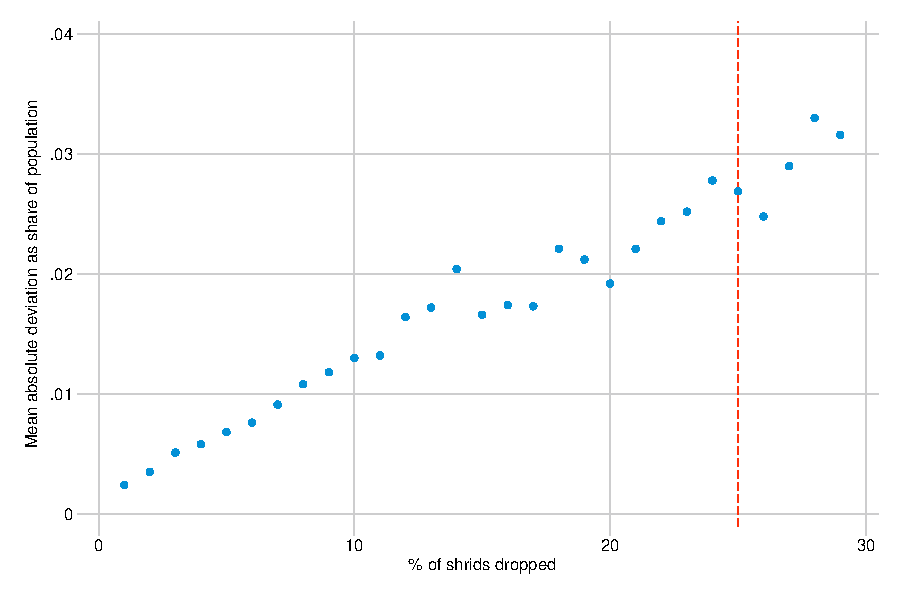
\includegraphics[scale=0.7]{\shrugpath/impute_sim_mad} \\
    \panel{B. Signed Imputation Error} \\
    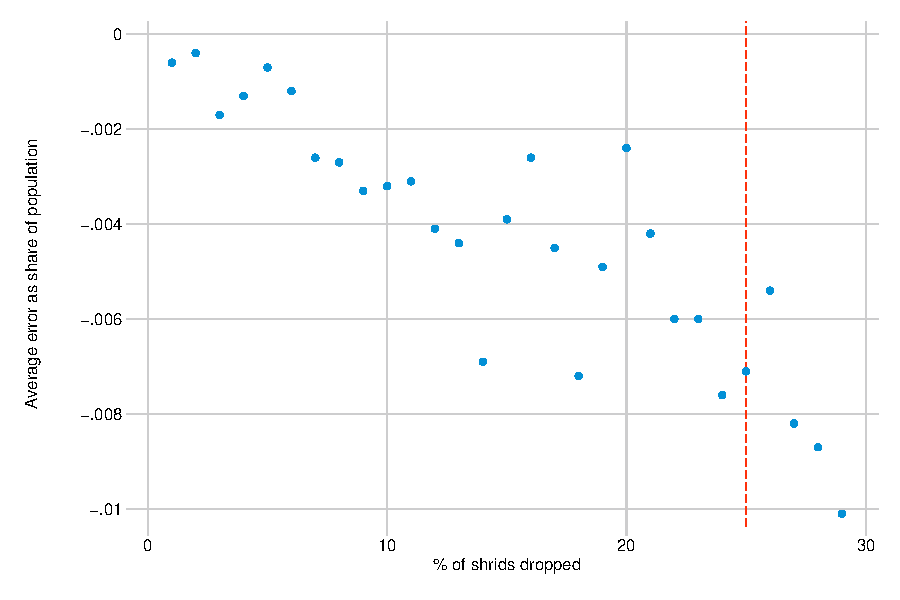
\includegraphics[scale=0.7]{\shrugpath/impute_sim_error} \\
  \end{tabular}
  
  \end{center}
  \begin{adjustwidth}{2cm}{2cm}
    \scriptsize{\textit{Source}: Authors' analysis based on data in
      the \href{http://www.devdatalab.org/shrug}{Socioeconomic
        High-resolution Rural-Urban Geographic Dataset on
        India}. \\ \textit{Note}: Panel A of
      Figure~\ref{fig:impute_error} shows the mean absolute deviation
      of simulated estimates of constitutency population as compared
      with actual constituency population, under scenarios where we
      set a different share of the population to missing. We run a
      simulation where before calculating constituency population, we
      drop village and town observations representing X\% of
      constituency population, and then use our imputation
      methodology. The graph shows, for instance, that when we drop
      20\% of the data before imputation, our average constituency has
      a total population error of approximately 1.8\%. Panel B shows
      the signed error rather than the absolute error, indicating a
      very small downward bias in population estimation from our
      method.}
  \end{adjustwidth}
  \label{fig:impute_error}
\end{figure}

\end{appendix}
  
\end{document}
